\subsection{Arquitectura del cliente}

\begin{figure}[H]
\centerline{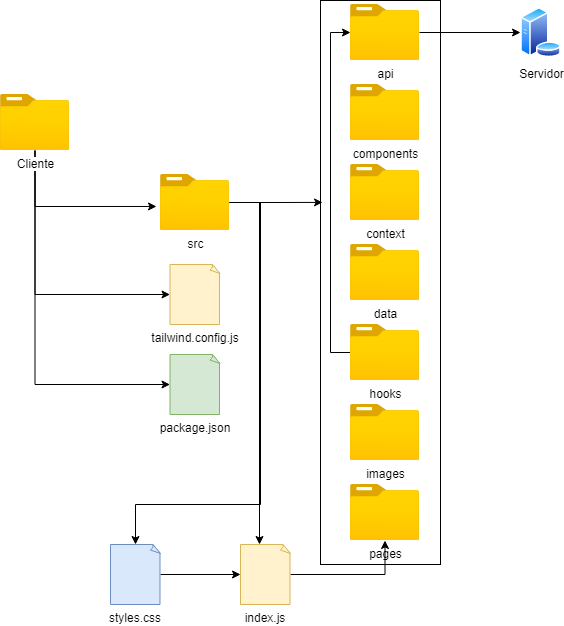
\includegraphics[width=15cm]{figuras/diseño/FicherosCliente.png}}
\caption{Arquitectura del cliente.}
\label{enlaceArquitecturaCliente}
\end{figure}

En la \hyperref[enlaceArquitecturaCliente]{Figura 3.4} se ilustra una pequeña representación de la arquitectura del cliente, con las diferentes partes que lo componen.
\\

En el cliente existen un total de ocho páginas: {\bf Edit}, {\bf NotFound}, {\bf Home}, {\bf Search}, {\bf Preview}, {\bf Save}, {\bf RegisterUsers} y {\bf Login}. Todas estas páginas son divididas en componentes, los cuales se almacenan en {\bf components} (no se ilustran en esta imagen de la arquitectura porque son más de 50). Estos componentes son estructuras de código más pequeñas, que, en conjunto, llegan a formar las páginas mencionadas anteriormente.
\\

Las distintas partes de las páginas, así como las propias páginas, hacen uso de los componentes de {\it data}, es decir, los mostrados en el cuadro amarillo. Estos son componentess que permiten automatizar el listado de selección de campos de cabecera, como puede ser el organismo de una ley, la sección a la que pertenece, el colectivo que lo publica, etc.
\\

En cuanto a las páginas, estas hacen uso del componente {\bf hooks} para poder llegar a establecer conexión con los datos del servidor. Las páginas hacen un llamamiento a {\it hooks}, que a su vez realiza un llamamiento al componente {\bf api}, el cual establece una interfaz con todas las solicitudes HTTP realizadas al servidor. Este componente realiza las solicitudes al servidor en primera instancia, y recibe la respuesta correspondiente del servidor, la cual se envía de vuelta hasta la página correspondiente, siguiendo el camino inverso.
\\

Existe un caso especial con respecto al párrafo anterior. Cuando se realiza la operación de inicio de sesión, esta se realiza en la página de Login. En este caso, se hace un llamamiento al componente {\bf auth} del {\it context}. Este componente se encarga de gestionar el almacenamiento local en la parte del cliente. Aquí se almacena, por ejemplo, el token JWT que fue enviado desde el servidor al realizar el inicio de sesión. De esta forma, en todo momento el usuario dispone del token necesario para realizar las operaciones que desee al estar autenticado.